% $Author: oscar $
% $Date: 2009-09-15 16:53:48 +0200 (Tue, 15 Sep 2009) $
% $Revision: 29111 $
%=================================================================
\ifx\wholebook\relax\else
% --------------------------------------------
% Lulu:
	\documentclass[a4paper,10pt,twoside]{book}
	\usepackage[
		papersize={6.13in,9.21in},
		hmargin={.815in,.815in},
		vmargin={.98in,.98in},
		ignoreheadfoot
	]{geometry}
	\usepackage[hangul]{kotex}
	% $Author: oscar $
% $Date: 2009-09-13 20:58:29 +0200 (Sun, 13 Sep 2009) $
% $Revision: 29070 $
%=============================================================
% NB: documentclass must be set in main document.
% Allows book to be generated in multiple formats.
%=============================================================
%:Packages
\usepackage[T1]{fontenc}  %%%%%really important to get the code directly in the text!
\usepackage{palatino}
\usepackage{ifthen}
\usepackage{graphicx}
\graphicspath{{figures/}}
\usepackage{xspace}
\usepackage{makeidx}
\usepackage{isodateo} % enable \isodate
\usepackage{amssymb,textcomp}
%=============================================================
%:More packages
%\usepackage[english]{babel}
%\usepackage{lmodern}
%\usepackage[scaled=0.85]{helvet}
%\usepackage{microtype}
%\usepackage{theorem}
%\usepackage{float}
%\usepackage{longtable}
%\usepackage[nottoc]{tocbibind}
%\usepackage{multicol}
%\usepackage{booktabs}	% book-style tables
%\usepackage{topcapt}	% enables \topcaption
%\usepackage{multirow}
%\usepackage{tabularx}
%\usepackage{alltt}
\usepackage[usenames,dvipsnames]{color}
%\usepackage[hang]{subfigure}\makeatletter\def\p@subfigure{\thefigure\,}\makeatother
%\usepackage{rotating}
%\usepackage{enumitem}	% apb: allows more control over tags in enumerations
%\usepackage{verbatim}     % for comment environment
%\usepackage{varioref}	% for page references that work
%\usepackage{needspace}
%\usepackage[newparttoc]{titlesec}
%\usepackage{titletoc}
%\usepackage{wrapfig}
\usepackage[
	colorlinks=true,
	linkcolor=black,
	urlcolor=black,
	citecolor=black
]{hyperref}   % should come last
%=============================================================
%:URL style
\makeatletter
\def\url@leostyle{%
  \@ifundefined{selectfont}{\def\UrlFont{\sf}}{\def\UrlFont{\sffamily}}}
\makeatother
\urlstyle{leo}
%=============================================================
%:Booleans
\newboolean{lulu}
\setboolean{lulu}{false}
\newcommand{\ifluluelse}[2]{\ifthenelse{\boolean{lulu}}{#1}{#2}}
%=============================================================
%:Editorial comment macros
\newcommand{\nnbb}[2]{
  \fbox{\bfseries\sffamily\scriptsize#1}
  {\sf\small$\blacktriangleright$\textit{#2}$\blacktriangleleft$}
}
\newcommand{\on}[1]{\nnbb{Oscar}{#1}}
\newcommand{\here}{\nnbb{CONTINUE}{HERE}}
%=============================================================
%:Abbreviation macros
\newcommand{\ie}{\emph{i.e.},\xspace}
\newcommand{\eg}{\emph{e.g.},\xspace}
\newcommand{\etc}{\emph{etc.}\xspace}
\newcommand{\etal}{\emph{et al.}\xspace}
\newcommand{\straightquote}{"}
\newcommand{\sba}{\url{SquareBracketAssociates.org}\xspace}
%=============================================================
%:Patterns
% \newcommand{\pattern}[2]{\newpage\section{{\sf #1}}\label{pat:#2}}
% \newcommand{\pattern}[2]{\newpage\index{#1 (Pattern)}\section{#1}\label{pat:#2}}
\newcommand{\pattern}[2]{\cleardoublepage\index{#1 (패턴)}\section{#1}\label{pat:#2}}
\newcommand{\thumbnail}[2]{\index{#1 (패턴)}\subsection{#1}\label{pat:#2}}
\newcommand{\thumblang}[2]{\index{#1 (패턴 랭귀지)}\subsection{#1}\label{pat:#2}}
\newcommand{\variant}[1]{{\emph{#1}}\xspace}
% \newcommand{\problem}[1]{\subsection*{Problem}\emph{#1}}
\newcommand{\intent}[1]{\paragraph{의도}\emph{#1}}
\newcommand{\problem}[1]{\paragraph{문제}\emph{#1}}
\newcommand{\solution}[1]{\paragraph{해결}\emph{#1}}
\newcommand{\discussion}[0]{\paragraph{토론}}
\newcommand{\cmd}[1]{{\tt #1}\xspace}
%=============================================================
%:Environments
\newenvironment{bulletlist}{\begin{itemize}\setlength{\itemsep}{0ex}}
{\end{itemize}}
%=============================================================
%:Cross reference macros
\newcommand{\chalabel}[1]{\label{cha:#1}}
\newcommand{\seclabel}[1]{\label{sec:#1}}
\newcommand{\figlabel}[1]{\label{fig:#1}}
\newcommand{\tablabel}[1]{\label{tab:#1}}
\newcommand{\rulelabel}[1]{\label{rule:#1}}
\newcommand{\eglabel}[1]{\label{eg:#1}}
\newcommand{\scrlabel}[1]{\label{scr:#1}}
\newcommand{\mthlabel}[1]{\label{mth:#1}}
\newcommand{\clslabel}[1]{\label{cls:#1}}
\newcommand{\faqlabel}[1]{\label{faq:#1}}
%\newcommand{\charef}[1]{Chapter~\ref{cha:#1}\xspace}
%\newcommand{\secref}[1]{Section~\ref{sec:#1}\xspace}
\newcommand{\figref}[1]{Figure~\ref{fig:#1}\xspace}
% \newcommand{\patpgref}[2]{\hyperref[pat:#2]{\sf #1} [p.~\pageref{pat:#2}]\xspace}
\newcommand{\patpgref}[2]{\index{#1 (Pattern)}\hyperref[pat:#2]{#1} [p.~\pageref{pat:#2}]\xspace}
\newcommand{\patlangpgref}[2]{\index{#1 (Pattern language)}\hyperref[pat:#2]{#1} [p.~\pageref{pat:#2}]\xspace}
% \newcommand{\patref}[2]{\hyperref[pat:#2]{\sf #1}\xspace}
\newcommand{\patref}[2]{\index{#1 (Pattern)}\hyperref[pat:#2]{#1}\xspace}
\newcommand{\patlangref}[2]{\index{#1 (Pattern language)}\hyperref[pat:#2]{#1}\xspace}
% \newcommand{\charef}[2]{\hyperref[cha:#2]{\underline{\sf #1}}\xspace}
% \newcommand{\charef}[2]{\hyperref[cha:#2]{\sf #1}\xspace}
\newcommand{\charef}[2]{\index{#1 (Pattern cluster)}\hyperref[cha:#2]{#1}\xspace}
% \newcommand{\chapgref}[2]{\hyperref[cha:#2]{\sf #1} [p.~\pageref{cha:#2}]\xspace}
\newcommand{\chapgref}[2]{\index{#1 (Pattern cluster)}\hyperref[cha:#2]{#1} [p.~\pageref{cha:#2}]\xspace}
%\newcommand{\Figref}[1]{Figure~\ref{fig:#1}\xspace}
%\newcommand{\appref}[1]{Appendix~\ref{app:#1}\xspace}
%\newcommand{\tabref}[1]{Table~\ref{tab:#1}\xspace}
%\newcommand{\ruleref}[1]{\ref{rule:#1}\xspace}
%\newcommand{\egref}[1]{example~\ref{eg:#1}\xspace}
%\newcommand{\Egref}[1]{Example~\ref{eg:#1}\xspace}
%\newcommand{\scrref}[1]{script~\ref{scr:#1}\xspace}
%\newcommand{\Scrref}[1]{Script~\ref{scr:#1}\xspace}
%\newcommand{\tscrref}[1]{the script~\ref{scr:#1}\xspace}
%\newcommand{\Tscrref}[1]{The script~\ref{scr:#1}\xspace}
%\newcommand{\mthref}[1]{method~\ref{mth:#1}\xspace}
%\newcommand{\mthsref}[1]{methods~\ref{mth:#1}\xspace}
%\newcommand{\Mthref}[1]{Method~\ref{mth:#1}\xspace}
%\newcommand{\tmthref}[1]{the method~\ref{mth:#1}\xspace}
%\newcommand{\Tmthref}[1]{The method~\ref{mth:#1}\xspace}
%\newcommand{\clsref}[1]{class~\ref{cls:#1}\xspace}
%\newcommand{\tclsref}[1]{the class~\ref{cls:#1}\xspace}
%\newcommand{\Tclsref}[1]{The class~\ref{cls:#1}\xspace}
%=============================================================
%:Page Layout
\setlength{\headsep}{1cm}
%=============================================================
%:Menu item macro
%\definecolor{lightgray}{gray}{0.89}
%\newcommand{\menu}[1]{{%
%	\setlength{\fboxsep}{0pt}%
%	\colorbox{lightgray}{{{\upshape\sffamily\strut \,#1\,}}}}}
%\newcommand{\go}{\,$\triangleright$\,}
%\newcommand{\short}[1]{\mbox{{\sc cmd}\hspace{0.08em}--\hspace{0.09em}#1}\xspace}
%\newcommand{\button}[1]{{%
%	\setlength{\fboxsep}{0pt}%
%	\fbox{{\upshape\sffamily\strut \,#1\,}}}}
%\newcommand{\toolsflap}{\textit{Tools} flap\xspace}
%=============================================================
%:Section depth
%\setcounter{secnumdepth}{2}
%
%\DeclareGraphicsExtensions{.pdf, .jpg, .png}
%=============================================================
%:PDF setup
\hypersetup{
   pdftitle={Object-Oriented Reengineering Patterns},
   pdfauthor={Serge Demeyer, St\'ephane Ducasse, Oscar Nierstrasz},
   pdfkeywords={Reengineering, Object-Oriented Programming, Patterns},
   pdfsubject={Computer Science}
}
%=============================================================
%:Page layout and appearance
%\renewcommand{\chaptermark}[1]{\markboth{#1}{}}
%\renewcommand{\sectionmark}[1]{\markright{\thesection\ #1}}
%\renewpagestyle{plain}[\small\itshape]{%
%	\setheadrule{0pt}%
%	\sethead[][][]{}{}{}%
%	\setfoot[][][]{}{}{}}
%\renewpagestyle{headings}[\small\itshape]{%
%	\setheadrule{0pt}%
%	\setmarks{chapter}{section}%
%	\sethead[\thepage][][\chaptertitle]{\sectiontitle}{}{\thepage}%
%	\setfoot[][][]{}{}{}}
%=============================================================
%:Title section setup and TOC numbering depth
%\setcounter{secnumdepth}{1}
%\setcounter{tocdepth}{1}
%\titleformat{\part}[display]{\centering}{\huge\partname\ \thepart}{1em}{\Huge\textbf}[]
%\titleformat{\chapter}[display]{}{\huge\chaptertitlename\ \thechapter}{1em}{\Huge\raggedright\textbf}[]
%\titlecontents{part}[3pc]{%
%		\pagebreak[2]\addvspace{1em plus.4em minus.2em}%
%		\leavevmode\large\bfseries}
%	{\contentslabel{3pc}}{\hspace*{-3pc}}
%	{}[\nopagebreak]
%\titlecontents{chapter}[3pc]{%
%		\pagebreak[0]\addvspace{1em plus.2em minus.2em}%
%		\leavevmode\bfseries}
%	{\contentslabel{3pc}}{}
%	{\hfill\contentspage}[\nopagebreak]
%\dottedcontents{section}[3pc]{}{3pc}{1pc}
%\dottedcontents{subsection}[3pc]{}{0pc}{1pc}
%\let\origdoublepage\cleardoublepage
%\newcommand{\clearemptydoublepage}{%
%  \clearpage
%  {\pagestyle{empty}\origdoublepage}}
%\let\cleardoublepage\clearemptydoublepage % see http://www.tex.ac.uk/cgi-bin/texfaq2html?label=patch
%=============================================================
%:Listings package configuration
\newcommand{\caret}{\makebox{\raisebox{0.4ex}{\footnotesize{$\wedge$}}}}
% \newcommand{\escape}{{\sf \textbackslash}}
\definecolor{source}{gray}{0.95}
\usepackage{listings}
\lstdefinelanguage{Smalltalk}{
  morestring=[d]',
% Adapt this to other languages!
%  morecomment=[s]{"}{"},
  alsoletter={\#:},
  %escapechar={!},
  literate=
    {BANG}{!}1
%    {UNDERSCORE}{\_}1
    {\\st}{Smalltalk}9 % convenience -- in case \st occurs in code
    % {'}{{\textquotesingle}}1 % replaced by upquote=true in \lstset
%    {_}{{$\leftarrow$}}1
    {>>>}{{\sep}}1
    {^}{{$\uparrow$}}1
    {~}{{$\sim$}}1
    {-}{{\sf -\hspace{-0.13em}-}}1  % the goal is to make - the same width as +
    {+}{\raisebox{0.08ex}{+}}1		% and to raise + off the baseline to match -
    {-->}{{\quad$\longrightarrow$\quad}}3
	, % Don't forget the comma at the end!
  tabsize=4
}[keywords,comments,strings]

\lstset{language=Smalltalk,
	basicstyle=\sffamily,
	keywordstyle=\color{black}\bfseries,
	% stringstyle=\ttfamily, % Ugly! do we really want this? -- on
	mathescape=true,
	showstringspaces=false,
	keepspaces=true,
	breaklines=true,
	breakautoindent=true,
	backgroundcolor=\color{source},
	lineskip={-1pt}, % Ugly hack
	upquote=true, % straight quote; requires textcomp package
	columns=fullflexible} % no fixed width fonts
% \newcommand{\ct}{\lstinline[mathescape=false,basicstyle={\sffamily\upshape}]}
\newcommand{\ct}{\lstinline[mathescape=false,backgroundcolor=\color{white},basicstyle={\sffamily\upshape}]}
\newcommand{\lct}[1]{{\textsf{\textup{#1}}}}
%\newcommand{\scat}[1]{\emph{\textsf{#1}}\xspace}
%\newcommand{\prot}[1]{\emph{\textsf{#1}}\xspace}
% NB: No argument!
\lstnewenvironment{code}[0]{%
	\lstset{%
		% frame=lines,
		frame=single,
		framerule=0pt,
		mathescape=false
	}
}{}
%\def\ignoredollar#1{}
%=============================================================
%:Reserving space
%\newcommand{\needlines}[1]{\Needspace{#1\baselineskip}}
%=============================================================
%:Indexing macros
% Macros ending with "ind" generate text as well as an index entry
% Macros ending with "index" *only* generate an index entry
\newcommand{\ind}[1]{\index{#1}#1\xspace} % plain text
\newcommand{\subind}[2]{\index{#1!#2}#2\xspace} % show #2, subindex under #1
\newcommand{\emphind}[1]{\index{#1}\emph{#1}\xspace} % emph #1
\newcommand{\emphsubind}[2]{\index{#1!#2}\emph{#2}\xspace} % show emph #2, subindex under #1
\newcommand{\patind}[1]{\index{#1@#1 (pattern)}\ct{#1}\xspace} % pattern
\newcommand{\seeindex}[2]{\index{#1|see{#2}}} % #1, see #2
%\newcommand{\boldidx}[1]{{\bf #1}} % breaks hyperlink
%\newcommand{\indmain}[1]{\index{#1}#1\xspace} 
%\newcommand{\emphsubindmain}[2]{\index{#1!#2}\emph{#2}\xspace} % subindex, main entry
%\newcommand{\subindmain}[2]{\index{#1!#2}#2\xspace} % subindex, main entry
%\newcommand{\clsindmain}[1]{\index{#1!\#@(class)}\ct{#1}\xspace} % class main
%\newcommand{\indexmain}[1]{\index{#1}} 
%=============================================================
\parskip 1ex
%=============================================================

	\pagestyle{headings}
	\setboolean{lulu}{true}
% --------------------------------------------
% A4:
%	\documentclass[a4paper,11pt,twoside]{book}
%	% $Author: oscar $
% $Date: 2009-09-13 20:58:29 +0200 (Sun, 13 Sep 2009) $
% $Revision: 29070 $
%=============================================================
% NB: documentclass must be set in main document.
% Allows book to be generated in multiple formats.
%=============================================================
%:Packages
\usepackage[T1]{fontenc}  %%%%%really important to get the code directly in the text!
\usepackage{palatino}
\usepackage{ifthen}
\usepackage{graphicx}
\graphicspath{{figures/}}
\usepackage{xspace}
\usepackage{makeidx}
\usepackage{isodateo} % enable \isodate
\usepackage{amssymb,textcomp}
%=============================================================
%:More packages
%\usepackage[english]{babel}
%\usepackage{lmodern}
%\usepackage[scaled=0.85]{helvet}
%\usepackage{microtype}
%\usepackage{theorem}
%\usepackage{float}
%\usepackage{longtable}
%\usepackage[nottoc]{tocbibind}
%\usepackage{multicol}
%\usepackage{booktabs}	% book-style tables
%\usepackage{topcapt}	% enables \topcaption
%\usepackage{multirow}
%\usepackage{tabularx}
%\usepackage{alltt}
\usepackage[usenames,dvipsnames]{color}
%\usepackage[hang]{subfigure}\makeatletter\def\p@subfigure{\thefigure\,}\makeatother
%\usepackage{rotating}
%\usepackage{enumitem}	% apb: allows more control over tags in enumerations
%\usepackage{verbatim}     % for comment environment
%\usepackage{varioref}	% for page references that work
%\usepackage{needspace}
%\usepackage[newparttoc]{titlesec}
%\usepackage{titletoc}
%\usepackage{wrapfig}
\usepackage[
	colorlinks=true,
	linkcolor=black,
	urlcolor=black,
	citecolor=black
]{hyperref}   % should come last
%=============================================================
%:URL style
\makeatletter
\def\url@leostyle{%
  \@ifundefined{selectfont}{\def\UrlFont{\sf}}{\def\UrlFont{\sffamily}}}
\makeatother
\urlstyle{leo}
%=============================================================
%:Booleans
\newboolean{lulu}
\setboolean{lulu}{false}
\newcommand{\ifluluelse}[2]{\ifthenelse{\boolean{lulu}}{#1}{#2}}
%=============================================================
%:Editorial comment macros
\newcommand{\nnbb}[2]{
  \fbox{\bfseries\sffamily\scriptsize#1}
  {\sf\small$\blacktriangleright$\textit{#2}$\blacktriangleleft$}
}
\newcommand{\on}[1]{\nnbb{Oscar}{#1}}
\newcommand{\here}{\nnbb{CONTINUE}{HERE}}
%=============================================================
%:Abbreviation macros
\newcommand{\ie}{\emph{i.e.},\xspace}
\newcommand{\eg}{\emph{e.g.},\xspace}
\newcommand{\etc}{\emph{etc.}\xspace}
\newcommand{\etal}{\emph{et al.}\xspace}
\newcommand{\straightquote}{"}
\newcommand{\sba}{\url{SquareBracketAssociates.org}\xspace}
%=============================================================
%:Patterns
% \newcommand{\pattern}[2]{\newpage\section{{\sf #1}}\label{pat:#2}}
% \newcommand{\pattern}[2]{\newpage\index{#1 (Pattern)}\section{#1}\label{pat:#2}}
\newcommand{\pattern}[2]{\cleardoublepage\index{#1 (패턴)}\section{#1}\label{pat:#2}}
\newcommand{\thumbnail}[2]{\index{#1 (패턴)}\subsection{#1}\label{pat:#2}}
\newcommand{\thumblang}[2]{\index{#1 (패턴 랭귀지)}\subsection{#1}\label{pat:#2}}
\newcommand{\variant}[1]{{\emph{#1}}\xspace}
% \newcommand{\problem}[1]{\subsection*{Problem}\emph{#1}}
\newcommand{\intent}[1]{\paragraph{의도}\emph{#1}}
\newcommand{\problem}[1]{\paragraph{문제}\emph{#1}}
\newcommand{\solution}[1]{\paragraph{해결}\emph{#1}}
\newcommand{\discussion}[0]{\paragraph{토론}}
\newcommand{\cmd}[1]{{\tt #1}\xspace}
%=============================================================
%:Environments
\newenvironment{bulletlist}{\begin{itemize}\setlength{\itemsep}{0ex}}
{\end{itemize}}
%=============================================================
%:Cross reference macros
\newcommand{\chalabel}[1]{\label{cha:#1}}
\newcommand{\seclabel}[1]{\label{sec:#1}}
\newcommand{\figlabel}[1]{\label{fig:#1}}
\newcommand{\tablabel}[1]{\label{tab:#1}}
\newcommand{\rulelabel}[1]{\label{rule:#1}}
\newcommand{\eglabel}[1]{\label{eg:#1}}
\newcommand{\scrlabel}[1]{\label{scr:#1}}
\newcommand{\mthlabel}[1]{\label{mth:#1}}
\newcommand{\clslabel}[1]{\label{cls:#1}}
\newcommand{\faqlabel}[1]{\label{faq:#1}}
%\newcommand{\charef}[1]{Chapter~\ref{cha:#1}\xspace}
%\newcommand{\secref}[1]{Section~\ref{sec:#1}\xspace}
\newcommand{\figref}[1]{Figure~\ref{fig:#1}\xspace}
% \newcommand{\patpgref}[2]{\hyperref[pat:#2]{\sf #1} [p.~\pageref{pat:#2}]\xspace}
\newcommand{\patpgref}[2]{\index{#1 (Pattern)}\hyperref[pat:#2]{#1} [p.~\pageref{pat:#2}]\xspace}
\newcommand{\patlangpgref}[2]{\index{#1 (Pattern language)}\hyperref[pat:#2]{#1} [p.~\pageref{pat:#2}]\xspace}
% \newcommand{\patref}[2]{\hyperref[pat:#2]{\sf #1}\xspace}
\newcommand{\patref}[2]{\index{#1 (Pattern)}\hyperref[pat:#2]{#1}\xspace}
\newcommand{\patlangref}[2]{\index{#1 (Pattern language)}\hyperref[pat:#2]{#1}\xspace}
% \newcommand{\charef}[2]{\hyperref[cha:#2]{\underline{\sf #1}}\xspace}
% \newcommand{\charef}[2]{\hyperref[cha:#2]{\sf #1}\xspace}
\newcommand{\charef}[2]{\index{#1 (Pattern cluster)}\hyperref[cha:#2]{#1}\xspace}
% \newcommand{\chapgref}[2]{\hyperref[cha:#2]{\sf #1} [p.~\pageref{cha:#2}]\xspace}
\newcommand{\chapgref}[2]{\index{#1 (Pattern cluster)}\hyperref[cha:#2]{#1} [p.~\pageref{cha:#2}]\xspace}
%\newcommand{\Figref}[1]{Figure~\ref{fig:#1}\xspace}
%\newcommand{\appref}[1]{Appendix~\ref{app:#1}\xspace}
%\newcommand{\tabref}[1]{Table~\ref{tab:#1}\xspace}
%\newcommand{\ruleref}[1]{\ref{rule:#1}\xspace}
%\newcommand{\egref}[1]{example~\ref{eg:#1}\xspace}
%\newcommand{\Egref}[1]{Example~\ref{eg:#1}\xspace}
%\newcommand{\scrref}[1]{script~\ref{scr:#1}\xspace}
%\newcommand{\Scrref}[1]{Script~\ref{scr:#1}\xspace}
%\newcommand{\tscrref}[1]{the script~\ref{scr:#1}\xspace}
%\newcommand{\Tscrref}[1]{The script~\ref{scr:#1}\xspace}
%\newcommand{\mthref}[1]{method~\ref{mth:#1}\xspace}
%\newcommand{\mthsref}[1]{methods~\ref{mth:#1}\xspace}
%\newcommand{\Mthref}[1]{Method~\ref{mth:#1}\xspace}
%\newcommand{\tmthref}[1]{the method~\ref{mth:#1}\xspace}
%\newcommand{\Tmthref}[1]{The method~\ref{mth:#1}\xspace}
%\newcommand{\clsref}[1]{class~\ref{cls:#1}\xspace}
%\newcommand{\tclsref}[1]{the class~\ref{cls:#1}\xspace}
%\newcommand{\Tclsref}[1]{The class~\ref{cls:#1}\xspace}
%=============================================================
%:Page Layout
\setlength{\headsep}{1cm}
%=============================================================
%:Menu item macro
%\definecolor{lightgray}{gray}{0.89}
%\newcommand{\menu}[1]{{%
%	\setlength{\fboxsep}{0pt}%
%	\colorbox{lightgray}{{{\upshape\sffamily\strut \,#1\,}}}}}
%\newcommand{\go}{\,$\triangleright$\,}
%\newcommand{\short}[1]{\mbox{{\sc cmd}\hspace{0.08em}--\hspace{0.09em}#1}\xspace}
%\newcommand{\button}[1]{{%
%	\setlength{\fboxsep}{0pt}%
%	\fbox{{\upshape\sffamily\strut \,#1\,}}}}
%\newcommand{\toolsflap}{\textit{Tools} flap\xspace}
%=============================================================
%:Section depth
%\setcounter{secnumdepth}{2}
%
%\DeclareGraphicsExtensions{.pdf, .jpg, .png}
%=============================================================
%:PDF setup
\hypersetup{
   pdftitle={Object-Oriented Reengineering Patterns},
   pdfauthor={Serge Demeyer, St\'ephane Ducasse, Oscar Nierstrasz},
   pdfkeywords={Reengineering, Object-Oriented Programming, Patterns},
   pdfsubject={Computer Science}
}
%=============================================================
%:Page layout and appearance
%\renewcommand{\chaptermark}[1]{\markboth{#1}{}}
%\renewcommand{\sectionmark}[1]{\markright{\thesection\ #1}}
%\renewpagestyle{plain}[\small\itshape]{%
%	\setheadrule{0pt}%
%	\sethead[][][]{}{}{}%
%	\setfoot[][][]{}{}{}}
%\renewpagestyle{headings}[\small\itshape]{%
%	\setheadrule{0pt}%
%	\setmarks{chapter}{section}%
%	\sethead[\thepage][][\chaptertitle]{\sectiontitle}{}{\thepage}%
%	\setfoot[][][]{}{}{}}
%=============================================================
%:Title section setup and TOC numbering depth
%\setcounter{secnumdepth}{1}
%\setcounter{tocdepth}{1}
%\titleformat{\part}[display]{\centering}{\huge\partname\ \thepart}{1em}{\Huge\textbf}[]
%\titleformat{\chapter}[display]{}{\huge\chaptertitlename\ \thechapter}{1em}{\Huge\raggedright\textbf}[]
%\titlecontents{part}[3pc]{%
%		\pagebreak[2]\addvspace{1em plus.4em minus.2em}%
%		\leavevmode\large\bfseries}
%	{\contentslabel{3pc}}{\hspace*{-3pc}}
%	{}[\nopagebreak]
%\titlecontents{chapter}[3pc]{%
%		\pagebreak[0]\addvspace{1em plus.2em minus.2em}%
%		\leavevmode\bfseries}
%	{\contentslabel{3pc}}{}
%	{\hfill\contentspage}[\nopagebreak]
%\dottedcontents{section}[3pc]{}{3pc}{1pc}
%\dottedcontents{subsection}[3pc]{}{0pc}{1pc}
%\let\origdoublepage\cleardoublepage
%\newcommand{\clearemptydoublepage}{%
%  \clearpage
%  {\pagestyle{empty}\origdoublepage}}
%\let\cleardoublepage\clearemptydoublepage % see http://www.tex.ac.uk/cgi-bin/texfaq2html?label=patch
%=============================================================
%:Listings package configuration
\newcommand{\caret}{\makebox{\raisebox{0.4ex}{\footnotesize{$\wedge$}}}}
% \newcommand{\escape}{{\sf \textbackslash}}
\definecolor{source}{gray}{0.95}
\usepackage{listings}
\lstdefinelanguage{Smalltalk}{
  morestring=[d]',
% Adapt this to other languages!
%  morecomment=[s]{"}{"},
  alsoletter={\#:},
  %escapechar={!},
  literate=
    {BANG}{!}1
%    {UNDERSCORE}{\_}1
    {\\st}{Smalltalk}9 % convenience -- in case \st occurs in code
    % {'}{{\textquotesingle}}1 % replaced by upquote=true in \lstset
%    {_}{{$\leftarrow$}}1
    {>>>}{{\sep}}1
    {^}{{$\uparrow$}}1
    {~}{{$\sim$}}1
    {-}{{\sf -\hspace{-0.13em}-}}1  % the goal is to make - the same width as +
    {+}{\raisebox{0.08ex}{+}}1		% and to raise + off the baseline to match -
    {-->}{{\quad$\longrightarrow$\quad}}3
	, % Don't forget the comma at the end!
  tabsize=4
}[keywords,comments,strings]

\lstset{language=Smalltalk,
	basicstyle=\sffamily,
	keywordstyle=\color{black}\bfseries,
	% stringstyle=\ttfamily, % Ugly! do we really want this? -- on
	mathescape=true,
	showstringspaces=false,
	keepspaces=true,
	breaklines=true,
	breakautoindent=true,
	backgroundcolor=\color{source},
	lineskip={-1pt}, % Ugly hack
	upquote=true, % straight quote; requires textcomp package
	columns=fullflexible} % no fixed width fonts
% \newcommand{\ct}{\lstinline[mathescape=false,basicstyle={\sffamily\upshape}]}
\newcommand{\ct}{\lstinline[mathescape=false,backgroundcolor=\color{white},basicstyle={\sffamily\upshape}]}
\newcommand{\lct}[1]{{\textsf{\textup{#1}}}}
%\newcommand{\scat}[1]{\emph{\textsf{#1}}\xspace}
%\newcommand{\prot}[1]{\emph{\textsf{#1}}\xspace}
% NB: No argument!
\lstnewenvironment{code}[0]{%
	\lstset{%
		% frame=lines,
		frame=single,
		framerule=0pt,
		mathescape=false
	}
}{}
%\def\ignoredollar#1{}
%=============================================================
%:Reserving space
%\newcommand{\needlines}[1]{\Needspace{#1\baselineskip}}
%=============================================================
%:Indexing macros
% Macros ending with "ind" generate text as well as an index entry
% Macros ending with "index" *only* generate an index entry
\newcommand{\ind}[1]{\index{#1}#1\xspace} % plain text
\newcommand{\subind}[2]{\index{#1!#2}#2\xspace} % show #2, subindex under #1
\newcommand{\emphind}[1]{\index{#1}\emph{#1}\xspace} % emph #1
\newcommand{\emphsubind}[2]{\index{#1!#2}\emph{#2}\xspace} % show emph #2, subindex under #1
\newcommand{\patind}[1]{\index{#1@#1 (pattern)}\ct{#1}\xspace} % pattern
\newcommand{\seeindex}[2]{\index{#1|see{#2}}} % #1, see #2
%\newcommand{\boldidx}[1]{{\bf #1}} % breaks hyperlink
%\newcommand{\indmain}[1]{\index{#1}#1\xspace} 
%\newcommand{\emphsubindmain}[2]{\index{#1!#2}\emph{#2}\xspace} % subindex, main entry
%\newcommand{\subindmain}[2]{\index{#1!#2}#2\xspace} % subindex, main entry
%\newcommand{\clsindmain}[1]{\index{#1!\#@(class)}\ct{#1}\xspace} % class main
%\newcommand{\indexmain}[1]{\index{#1}} 
%=============================================================
\parskip 1ex
%=============================================================

%	\usepackage{a4wide}
% --------------------------------------------
	\begin{document}
	\renewcommand{\nnbb}[2]{} % Disable editorial comments
	\sloppy
\fi
%=================================================================
\chapter{테스트라는 생명보험}
\chalabel{TestsYourLifeInsurance}

여러분은 리엔지니어링 프로젝트의 시작 단계에 있다. 여러분은 소중한 레거시 시스템의 많은 부분에 대해 근본적인 수술을 수행해야 한다는 것을 알고 있다. 비즈니스가 의존하는 시스템을 변경할 때 발생하는 위험, 즉 기존에 작동하던 \emph{기능이 중단될 위험}, \emph{잘못된 작업에 너무 많은 노력을 기울일 위험}, \emph{필요한 새 기능을 시스템에 통합하지 못할 위험}, \emph{유지보수 비용이 증가할 위험}을 어떻게 최소화할 수 있을지 고민하고 있을 것이다.
\index{테스팅}

이 클러스터에 제시된 패턴은 리엔지니어링 변경으로 인한 위험을 줄이기 위해 리엔지니어링 컨텍스트에서 테스트를 사용하는 효과적인 방법을 제시한다.

\noindent
\emph{경고.}
테스트는 이 장에서 몇 페이지에 걸쳐 자세히 다룰 수 없을 정도로 풍부하고 중요한 주제이다. 리엔지니어링 프로젝트와 특히 관련이 있는 몇 가지 중요한 테스트 패턴을 파악하고 몇 가지 주요 이슈를 간략하게만 설명할 것이다. 예를 들어, 바인더는 책 전체를 객체 지향 시스템 테스트에 할애하고 있다 \cite{Bind99a}.
\index{빈더, 로버트}

\subsection*{포스: 주요한 요구사항}

이러한 패턴은 레거시 시스템의 진화에 대한 다양한 위험 요소와 관련된 공통적인 포스를 공유한다. 각 패턴은 노력과 리스크 사이의 일정한 균형을 달성하기 위해 이러한 주요 요구사항 중 일부를 해결한다.

\subsubsection*{리엔지니어링 포스}

\begin{bulletlist}
\item 레거시 시스템에는 테스트 절차가 정의되어 있지 않은 경우가 많다.

\item 새로운 버그가 발생하지 않고 시스템의 일부를 변경하는 것은 어려운 작업이다.
\end{bulletlist}

\subsubsection*{시스템 개발 포스}

\begin{bulletlist}
\item 시스템의 모든 측면을 테스트할 수 있는 것은 아니다.

\item 동시성(concurrency) 및 사용자 인터페이스와 같은 특정 측면은 테스트하기 어렵다.

\item 시간에 쫓기면 테스트 작성은 항상 가장 먼저 제거되는 작업이다.

\item 소수의 사람에게만 시스템에 대한 모든 지식이 집중되어 있으면 프로젝트의 미래에 큰 위험을 초래할 수 있다.
\end{bulletlist}

\subsubsection*{인적 측면 포스 (고객)}

\begin{bulletlist}
\item 고객은 궁극적으로 테스트 비용이 아니라 시스템의 새로운 기능에 대한 비용을 지불한다.

\item 불안정하거나 버그가 있는 시스템은 고객에게 허용되지 않는다.
\end{bulletlist}

\subsubsection*{인적 측면 포스 (개발자)}

\begin{bulletlist}
\item 프로그래머는 좋은 코드를 작성하기 때문에 테스트가 필요하지 않다고 생각한다. 

\item 프로그래머는 한 달 후 프로젝트를 떠날 수도 있기 때문에 장기적인 목표에 대해 동기 부여받지 않는다. 

\item 프로그래머는 문제를 파악하는 데 낭비되는 시간을 줄일 수 있는 도구와 프로세스에 더 관심이 많다.

\item 버그 수정은 재미가 없다.

\item 테스트 작성은 고급 작업으로 간주되지 않는다.
\end{bulletlist}

\subsection*{개요}

\begin{figure}
\begin{center}
\includegraphics[width=\textwidth]{TestingMap}
\caption{언제, 왜, 어떻게, 무엇을 테스트해야 하는가.}
\figlabel{TestingMap}
\end{center}
\end{figure}

\figref{TestingMap}에 표시된 것처럼, \patref{진화 활성화를 위한 테스트 작성하기}{WriteTestsToEnableEvolution}는 이 클러스터의 시작점이다. 이 클러스터는 리엔지니어링 프로젝트에 체계적인 테스트가 중요한 이유와 어떤 종류의 테스트가 필요한지 설명한다. 이 클러스터는 필요에 따라 새로운 테스트를 도입하는 전략을 옹호하는 \patref{기본 테스트를 증가시키기}{GrowYourTestBaseIncrementally}를 기반으로 한다.

테스트의 점진적 도입을 효과적으로 관리하려면 \patref{테스트 프레임워크 사용하기}{UseATestingFramework}를 사용하여 테스트 제품군을 구조화하고 구성하는 것이 중요하다. 테스트 프레임워크는 특정 스타일의 테스트를 설계하는 데 도움이 된다. 특히, 블랙박스 테스트 전략을 사용하여 구성 요소의 \patref{구현이 아닌 인터페이스 테스트하기}{TestTheInterfaceNotTheImplementation}를 수행하면 시스템 변경 시 테스트가 더 유용해지는 경향이 있다. 또한 \patref{비즈니스 규칙을 테스트로 기록}{RecordBusinessRulesAsTests}를 사용하면 급격한 변화가 있는 경우에도 비즈니스 규칙을 명시적으로 표현하고 실행 중인 시스템과 지속적으로 동기화할 수 있는 효과적인 방법을 확보할 수 있다.

테스트는 여러 가지 이유로 여러 시점에 도입될 수 있다. \patref{이해하기 위해 테스트 작성하기}{WriteTestsToUnderstand}은 변경 사항을 구현하기 위해 이해해야 하는 시스템 부분에 테스트 노력을 투자할 것을 권장한다. 보다 구체적으로는 \patref{퍼지 기능 테스트하기}{TestFuzzyFeatures}, \patref{오래된 버그 테스트하기}{TestOldBugs}, 특히 \patref{지속적인 문제 재테스트}{RetestPersistentProblems}를 사용하는 것이 좋다.

이 클러스터의 패턴은 리엔지니어링을 위해 \chapgref{마이그레이션 전략}{MigrationStrategies}를 직접 지원한다: \patpgref{변경할 때마다 회귀 테스트하기}{RegressionTestAfterEveryChange}는 시스템을 점진적으로 변경할 때마다 모든 것이 계속 실행되는지 확인하여 신뢰를 구축하는 데 도움이 됩니다. 사실상 이 테스트는 \patpgref{항상 실행 버전 보유하기}{AlwaysHaveARunningVersion}의 필수 전제 조건이며, 이를 통해 \patpgref{시스템 점진적 마이그레이션하기}{MigrateSystemsIncrementally}을 수행할 수 있다.

%=================================================================
%:PATTERN -- {Write Tests to Enable Evolution}
\pattern{진화 활성화를 위한 테스트 작성하기}{WriteTestsToEnableEvolution}

\intent{체계적인 테스트 프로그램을 적용해서 레거시 코드에 대한 투자를 보호하자.}

\subsection*{문제}

리엔지니어링 프로젝트의 리스크, 특히 다음과 같은 리스크를 어떻게 최소화할 수 있는가?

\begin{bulletlist}
\item 레거시 시스템을 단순화하지 못함.
\item 시스템에 더 많은 복잡성을 도입.
\item 기존에 작동하던 기능이 중단.
\item 잘못된 작업에 너무 많은 노력을 소비.
\item 향후 변화를 수용하지 못함.
\end{bulletlist}

\emph{이 문제는 다음과 같은 이유로 어렵다.}

\begin{bulletlist}
\item 시스템의 일부가 잘 이해되지 않거나 숨겨진 종속성이 있을 수 있으므로 변경의 영향을 항상 예측할 수 없다. 
\item 레거시 시스템을 변경하면 문서화되지 않은 측면이나 종속성으로 인해 시스템이 불안정해질 수 있다.
\end{bulletlist}

\emph{그러나 이 문제를 해결할 수 있는 이유는 다음과 같다.}

\begin{bulletlist}
\item 실행 중인 시스템이 있으므로 무엇이 작동하고 무엇이 작동하지 않는지 확인할 수 있다.
\item 시스템의 어떤 부분이 안정적이고 어떤 부분이 변경될 수 있는지 알 수 있다.
\end{bulletlist}

\subsection*{해결}

자동화되고 반복 가능하며 저장 가능한 테스트에 기반한 테스트 프로세스를 도입하자.
\subsubsection*{힌트}

Well-designed tests exhibit the following properties:

\begin{bulletlist}
\item \emph{자동화(Automation).} use them.
테스트는 사람의 개입 없이 실행되어야 한다. 완전 자동화된 테스트만이 시스템을 변경할 때마다 시스템이 이전과 동일하게 작동하는지 효율적으로 확인할 수 있는 방법을 제공한다. 테스트를 실행하는 데 필요한 노력을 최소화하면 개발자는 테스트 사용을 주저하지 않게 된다.

\item \emph{지속성(Persistence).}
테스트는 자동화할 수 있도록 저장되어야 한다. 각 테스트는 테스트 데이터, 수행할 작업 및 예상 결과를 문서화한다. 예상한 결과를 얻으면 테스트가 성공하고, 그렇지 않으면 실패한다. 저장된 테스트는 시스템이 작동할 것으로 예상되는 방식을 문서화한다.

\item \emph{반복성(Repeatability).}
변경 사항이 구현된 후 테스트를 반복할 수 있으면 시스템에 대한 신뢰도가 높아진다. 새로운 기능이 추가될 때마다 기존 테스트 풀에 새로운 테스트를 추가하여 시스템에 대한 신뢰도를 높일 수 있다.

\item \emph{유닛 테스트(Unit testing).}
테스트는 개별 소프트웨어 컴포넌트에 연결하여 시스템의 어느 부분을 테스트하는지 명확하게 식별할 수 있도록 해야 한다 \cite{Davi95a}.

\item \emph{독립성(Independence).}
각 테스트는 다른 테스트에 대한 종속성을 최소화해야 한다. 종속성이 높은 테스트는 일반적으로 하나의 테스트가 중단되면 다른 많은 테스트도 중단되는 눈사태 효과(avalanche effects)를 초래한다. 실패 횟수가 감지된 문제의 크기를 정량적으로 나타내는 것이 중요하다. 이렇게 하면 테스트에 대한 불신을 최소화할 수 있다. 프로그래머는 테스트를 믿어야 한다.
\end{bulletlist}

\subsection*{트레이드오프}

\subsubsection*{장점}

\begin{bulletlist}
\item 테스트는 시스템에 대한 신뢰도를 높이고 동작을 보존하는 방식으로 시스템의 기능, 디자인, 아키텍처까지 변경할 수 있는 능력을 향상시킨다.
\item 테스트는 시스템의 산출물을 사용하는 방법을 문서화한다. 일반적인 문서와 달리 동작하는 테스트는 시스템에 대한 항상 최신 설명을 제공한다.
\item 보안(security)과 안정성(stability)를 우려하는 고객에게 테스트에 대한 것을 판매의 포인트를 삼는 것은 일반적으로 문제가 되지 않는다. 시스템의 장기적인 수명의 보장에도 테스트는 좋은 이야기 거리가 될 수 있다.
\item 테스트는 향후 시스템 진화를 가능하게 하는 데 필요한 환경을 제공한다.
\item Smalltalk, Java, C++, 심지어 Perl과 같은 모든 주요 객체 지향 언어에 대한 간단한 단위 테스트 프레임워크가 존재한다.
\end{bulletlist}

\subsubsection*{단점}

\begin{bulletlist}
\item 테스트는 무료가 아니다. 테스트를 작성하려면 리소스를 할당해야 한다.
\item 테스트는 결함의 존재 여부만 입증할 수 있다. 레거시 시스템(또는 모든 시스템)의 모든 측면을 테스트하는 것은 불가능하다.
\item 불충분한 테스트는 잘못된 확신을 줄 수 있다. 모든 테스트가 실행되었기 때문에 시스템이 잘 작동한다고 생각할 수 있지만 전혀 그렇지 않을 수도 있다.
\end{bulletlist}

\subsubsection*{어려움}

\begin{bulletlist}
\item 수많은 테스트 접근 방식이 존재한다. 개발 프로세스에 맞는 간단한 접근 방식을 선택하자.
\item 레거시 시스템은 규모가 크고 문서화되지 않은 경향이 있기 때문에 테스트하기가 어렵다. 때때로 시스템의 일부를 테스트하려면 크고 복잡한 설정 절차가 필요하며, 이는 부담스러워 보일 수 있다.
\item 경영진이 테스트에 투자하는 것을 꺼릴 수 있다. 다음은 테스트에 찬성하는 몇 가지 근거이다.

\begin{bulletlist}
\item 테스트는 시스템의 안전성을 개선하는 데 도움이 됩니다. 

\item 테스트는 시스템 기능에 대한 확실한 신뢰를 보여준다.

\item 자동화된 테스트가 있으면 디버깅이 더 쉬워집니다.

\item 테스트는 애플리케이션과 항상 동기화되는 간단한 문서이다. 
\end{bulletlist}

\item 개발자는 테스트 도입을 꺼릴 수 있다. 테스트가 현재의 개발 속도를 높일 뿐만 아니라 향후 유지 관리 작업의 속도를 높일 수 있다는 비즈니스 사례를 구축하자. 버그를 수정하는 데 하루를 보낸 후 변경 사항이 유효한지 확인하는 데 3일을 더 소비하는 개발자와 이야기를 나눈 적이 있다. 자동화된 테스트가 일상 업무에서 프로그램을 더 빨리 디버깅하는 데 도움이 될 수 있다는 것을 보여 주자 그는 마침내 확신을 갖게 되었다.
\item 테스트는 개발자에게 지루할 수 있으므로 최소한 올바른 도구를 사용하자. 단위 테스트의 경우, SUnit과 그 다양한 변형은 간단하고 무료이며 Smalltalk, C++, Java 및 기타 언어 \cite{Beck98a}에서 사용할 수 있다.
\end{bulletlist}

\subsection*{예시}

다음 코드는 Java\cite{Beck98a}에서 \ind{JUnit}을 사용하여 작성한 단위 테스트를 보여준다. 이 테스트는 \lct{Money} 클래스에 정의된 \lct{add} 연산이 예상대로 작동하는지, 즉 \lct{12 CHF + 14 CHF = 26 CHF}가 되는지 확인한다.

\begin{code}
public class MoneyTest extends TestCase {
	public void testSimpleAdd() {
		Money m12CHF= new Money(12, "CHF");                 // (1)
		Money m14CHF= new Money(14, "CHF");        
		Money expected= new Money(26, "CHF");
		Money result= m12CHF.add(m14CHF);                     // (2)
		assert(result.currency().equals(expected.currency())
			&& result.amount() == expected.amount());            // (3)
	}
}
\end{code}

이는 테스트가 가져야 하는 다음 속성을 충족한다.

\begin{bulletlist}
\item 이 테스트는 자동화되어 있다. 동작이 올바른 경우 부울 값 참을 반환하고 그렇지 않으면 거짓을 반환한다.
\item 테스트가 저장된다. 테스트 클래스의 메서드이다. 따라서 다른 코드처럼 버전 관리가 가능한다.
\item 테스크가 반복 가능하다. 초기화 부분(1)은 테스트를 실행하고 무한히 재실행할 수 있는 컨텍스트를 생성한다. 
\item 다른 테스트와 독립적이다. 
\end{bulletlist}

이러한 속성을 가진 테스트를 사용하면 장기적으로 테스트 스위트(test suite)를 구축하는 데 도움이 된다. 버그를 수정하거나 새로운 기능을 추가한 후 또는 이미 존재하는 시스템 측면을 테스트하기 위해 테스트를 작성할 때마다 시스템에 대한 \emph{재현 가능(reproducible)} 및 \emph{검증 가능(verifiable)} 정보를 테스트 스위트에 추가하는 것이다. 특히 시스템 리엔지니어링의 맥락에서 이러한 재현 가능하고 검증 가능한 정보는 변경 후 시스템의 측면이 손상되었는지 확인할 수 있어 중요하다.

\subsection*{근거}

\begin{figure}[h]
\begin{center}
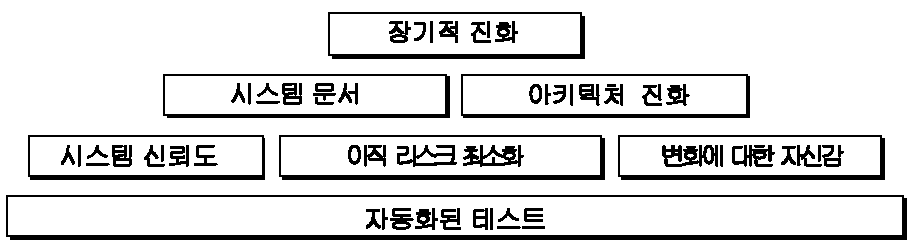
\includegraphics[width=\textwidth]{TestingFoundation}
\caption{자동화된 테스트는 리엔지니어링의 \emph{기반(foundation)}이다. 시스템에 대한 신뢰를 구축하고, 리스크를 줄이며, 시스템을 변경할 수 있는 능력에 대한 자신감을 높여준다.}
\figlabel{TestingFoundation}
\end{center}
\end{figure}

\noindent
테스트는 시스템의 일부가 \emph{검증 가능한(verifiable)} 방식으로 작동하는 방식을 지정하고 언제든지 실행하여 시스템이 여전히 일관적인지 확인할 수 있기 때문에 시스템에 대한 신뢰도를 나타낸다. 

\index{데이비스, 앨런}
\begin{quotation}
\noindent
\emph{``... 테스트는 단순히 프로그램에 결함이 있음을 드러낼 뿐 결함의 부재를 검증하는 데 사용할 수 없다. 프로그램이 올바르다는 신뢰도를 높일 수 있다.''}

\hfill --- 앨런 데이비스, 원칙 111 \cite{Davi95a}
\end{quotation}

체계적인 테스트는 \ind{익스트림 프로그래밍}\emph{(Extreme Programming)}에서 크게 장려한다. \cite{Beck00a} 변화하는 요구사항에 맞춰 프로그램을 신속하게 조정하는 데 필요한 기본 기술 중 하나이다. 레거시 시스템을 변경하는 것은 위험한 작업이다. 변경 후에도 코드가 계속 작동할까? 예상치 못한 부작용이 얼마나 많이 나타날까? 자동화되고 반복 가능한 일련의 테스트가 있으면 이러한 위험을 줄이는 데 도움이 된다. 

\begin{bulletlist}
\item 실행 가능한 테스트 세트는 시스템에 대한 신뢰도를 높여준다. (``이 코드가 정말 작동하는 게 확실한가요?'' ''네, 여기 이를 증명하는 테스트가 있어요.'')
\item 실행 중인 테스트 세트는 시스템에 대한 \emph{재현 가능(reproducible)}하고 \emph{검증 가능(verifiable)}한 정보를 나타내며, 애플리케이션과 항상 동기화되어 있다. 이는 일반적으로 다음 날이면 이미 약간 오래된 문서가 되는 대부분의 일반적인 문서와 대조적이다.
\item 테스트를 작성하면 개발 프로세스 초기에 버그를 발견할 수 있으므로 생산성이 향상된다.
\end{bulletlist}

\subsection*{관련 패턴}

\patref{진화 활성화를 위한 테스트 작성하기}{WriteTestsToEnableEvolution}는 \patpgref{항상 실행 버전 보유하기}{AlwaysHaveARunningVersion}의 전제 조건이다. 포괄적인 테스트 프로그램이 준비되어 있어야만 \patref{시스템 점진적 마이그레이션하기}{MigrateSystemsIncrementally}를 사용할 수 있다. 

\patref{기본 테스트를 증가시키기}{GrowYourTestBaseIncrementally} 및 \patref{구현이 아닌 인터페이스 테스트하기}{TestTheInterfaceNotTheImplementation}는 시스템이 진화하는 동안 테스트 스위트를 점진적으로 구축하는 방법을 소개한다. 

%=================================================================
%:PATTERN -- {Grow Your Test Base Incrementally}
\pattern{기본 테스트를 증가시키기}{GrowYourTestBaseIncrementally}


\intent{특정 시점에 필요한 테스트만 점진적으로 도입하여 테스트의 비용(cost)과 이점(benefit)을 균형 있게 조정한다.}

\subsection*{문제}

언제 테스트를 도입해야 하는가? 언제 중단할 수 있는가?

\emph{이 문제는 다음과 같은 이유로 어렵다.}

\begin{bulletlist}
\item 리엔지니어링 프로젝트에서는 테스트 작성에 너무 많은 시간을 할애할 여유가 없다.
\item 레거시 시스템은 방대한 경향이 있으므로 모든 것을 테스트하는 것은 불가능하다.
\item 레거시 시스템은 잘 문서화되어 있지 않고 잘 이해되지 않는 경향이 있다.
\item 시스템을 원래 개발했던 개발자는 떠났을 수 있고 시스템 유지 보수자는 시스템의 내부 작동에 대해 제한된 지식만 가지고 있을 수 있다.
\end{bulletlist}

\emph{그러나 이 문제를 해결할 수 있는 이유는 다음과 같다.}

\begin{bulletlist}
\item 우리는 취약한 부분이나 변경하고 싶은 부분이 어디에 있는지 알고 있다.
\item 우리는 프로그래머에게 테스트를 통해 이점을 얻을 수 있다고 설득할 수 있다.
\end{bulletlist}

\subsection*{해결}

작업 중인 시스템의 일부에 대해 테스트를 점진적으로 도입하자.

\subsubsection*{힌트}

\begin{bulletlist}
\item 우선순위를 신중하게 평가하고 처음에는 가장 중요한 구성 요소에 대해서만 테스트를 개발하자. 시스템을 리엔지니어링하면서 새로운 기능, 영향을 받을 수 있는 레거시 부분 및 그 과정에서 발견한 버그에 대한 테스트를 도입하자. 
\item 이전 시스템의 스냅샷을 잘 보관해 두면 나중에 원래 시스템과 새 버전 모두에 대해 실행해야 하는 테스트를 도입할 수 있다.
\item 비즈니스 가치에 집중하자. 시스템에서 가장 중요한 산출물이 있는 부분에 대한 테스트를 작성하기 시작하자. \patref{비즈니스 규칙을 테스트로 기록하기}{RecordBusinessRulesAsTests}를 시도해 보자.
\item 버그 수정 또는 문제에 대해 관리하고 있는 경우 \patref{오래된 버그 테스트하기}{TestOldBugs}를 시작점으로 적용하자.
\item 허용 가능한 문서와 시스템의 원 개발자가 있는 경우 \patpgref{퍼지 기능 테스트하기}{TestFuzzyFeatures}를 적용하는 것이 좋다.
\item \patref{구현이 아닌 인터페이스 테스트하기}{TestTheInterfaceNotTheImplementation}을 적용하고, 큰 추상화부터 테스트를 시작한 다음 시간이 허락한다면 테스트를 구체화하자. 예를 들어 파이프라인 아키텍처가 있는 경우 전체 파이프라인의 출력이 올바른 입력이 주어졌을 때 올바른지 확인하는 테스트를 작성하기 시작하자. 그런 다음 개별 파이프라인 컴포넌트에 대한 테스트를 작성하자.
\item 향후 구현이 변경될 가능성이 있는 부분(하위 시스템, 클래스, 메서드)을 블랙박스 테스트하자.
\index{블랙박스 테스트}
\end{bulletlist}

\subsection*{트레이드오프}

\subsubsection*{장점}

\begin{bulletlist}
\item 필요한 테스트만 개발하여 시간을 절약할 수 있다.
\item 프로젝트가 진행됨에 따라 가장 중요한 테스트의 기반을 구축할 수 있다.
\item 진행하면서 신뢰도를 높일 수 있다.
\item 향후 개발 및 유지 관리 활동을 간소화할 수 있다.
\end{bulletlist}

\subsubsection*{단점}

\begin{bulletlist}
\item 테스트해야 할 중요한 측면을 잘못 추측할 수 있다.
\item 테스트는 잘못된 확신을 줄 수 있다 --- 테스트되지 않은 버그가 여전히 시스템에 숨어 있을 수 있다.
\end{bulletlist}

\subsubsection*{어려움}

\begin{bulletlist}
\item 테스트에 적합한 컨텍스트를 설정하려면 상당한 시간과 노력이 필요할 수 있다.
\item 테스트할 구성 요소의 경계를 파악하는 것도 어렵다. 테스트할 부분과 테스트의 세분화 수준을 결정하려면 시스템과 리엔지니어링 방식을 잘 이해해야 한다.
\end{bulletlist}

\subsection*{예시}

\begin{figure}[h]
\begin{center}
\includegraphics[width=0.8\textwidth]{TestingChange}
\caption{변경하려는 시스템 부분에 대한 테스트를 도입.}
\figlabel{TestingChange}
\end{center}
\end{figure}

처음에는 변경하려는 하위 시스템 및 구성 요소에 대해서만 테스트를 도입한다. 하위 시스템 ABC와 그 컴포넌트 B에 대한 몇 가지 테스트를 도입하고, \patref{구현이 아닌 인터페이스 테스트하기}{TestTheInterfaceNotTheImplementation}을 적용하여 B에 대한 테스트가 newB에 대해서도 통과해야 한다는 것을 확인한다.

컴포넌트 B에 대한 테스트만 도입하면 A 및 C와의 통합을 테스트하지 못하므로 중요한 모든 측면을 테스트하지 못할 수 있으므로 버그가 발견되고 수정됨에 따라 점진적으로 새로운 테스트를 추가하는 것이 중요하다.

\subsection*{근거}

점진적 테스트 전략을 사용하면 모든 테스트가 완료되기 전에 리엔지니어링 작업을 시작할 수 있다. 현재 변경하려는 시스템 부분과 관련된 테스트에만 집중함으로써 테스트에 대한 최소한의 투자로 변경을 가능하게 하고, 테스트 기반을 확장하면서 팀이 자신감을 쌓을 수 있도록 도와준다.

\subsection*{관련 패턴}

\patref{테스트 프레임워크 사용하기}{UseATestingFramework}를 사용하여 테스트를 구조화 하자. 

\patref{구현이 아닌 인터페이스 테스트하기}{TestTheInterfaceNotTheImplementation}는 임의의 세부 수준에서 테스트를 개발하기 위한 전략을 제공한다. \patref{비즈니스 규칙을 테스트로 기록하기}{RecordBusinessRulesAsTests}는 비즈니스 로직을 구현하는 구성 요소를 테스트하기 위한 또 다른 전략을 제공한다. \patref{이해를 위해 테스트 작성하기}{WriteTestsToUnderstand}는 시스템을 리버스 엔지니어링하는 동안 테스트 기반을 준비할 수 있도록 도와준다.

%=================================================================
%:PATTERN -- {Use a Testing Framework}
\pattern{테스트 프레임워크 사용하기}{UseATestingFramework}

\intent{테스트를 쉽게 개발, 구성 및 실행할 수 있는 프레임워크를 제공하여 개발자가 회귀 테스트를 작성하고 사용하도록 장려한다.}

\subsection*{문제}

팀이 체계적인 테스트를 채택하도록 어떻게 장려하는가?

\emph{이 문제는 다음과 같은 이유로 어렵다.} 

\begin{bulletlist}
\item 테스트는 작성은 지루하다.
\item 테스트를 수행하려면 상당한 양의 테스트 데이터를 사용하기 위해 가져와야 할 수 있다.
\item 테스트 실패와 예기치 않은 오류를 구분하기 어려울 수 있다.
\end{bulletlist}

\emph{그러나 이 문제를 해결할 수 있는 이유는 다음과 같다.}

\begin{bulletlist}
\item 대부분의 테스트는 테스트 데이터를 생성하고, 몇 가지 작업을 수행하고, 결과가 예상과 일치하는지 확인하고, 테스트 데이터를 정리하는 등 동일한 기본 패턴을 따른다.
\item 테스트를 실행하고 실패 및 오류를 보고하는 데 필요한 인프라가 아주 적다.
\end{bulletlist}

\subsection*{해결}

개별 테스트 케이스에서 테스트 스위트를 구성할 수 있는 테스트 프레임워크를 사용한다.

\subsubsection*{단계}

\ind{JUnit} 및 \ind{SUnit}과 같은 단위 테스트 프레임워크\cite{Beck98a}와 같은 단위 테스트 프레임워크와 대부분의 프로그래밍 언어에 사용할 수 있는 다양한 상용 테스트 하네스 패키지가 있다. 사용 중인 프로그래밍 언어에 적합한 테스트 프레임워크를 사용할 수 없는 경우 다음 원칙에 따라 쉽게 직접 만들 수 있다.

\begin{bulletlist}
\item 사용자는 테스트 데이터를 설정하고, 실행하고, 결과에 대한 어설션(assertion)을 만드는 테스트 케이스를 제공해야 한다.
\item 테스트 프레임워크는 어설션(assertion) 실패와 예기치 않은 오류를 구분할 수 있는 테스트로 테스트 케이스를 래핑해야 한다.
\item 테스트 프레임워크는 테스트가 성공할 경우 최소한의 피드백만 제공해야 한다.

\begin{bulletlist}
\item 어설션(assertion) 실패는 어떤 테스트가 실패했는지 정확하게 표시해야 한다.

\item 오류는 더 자세한 피드백(예: 전체 스택 추적)을 제공해야 한다.
\end{bulletlist}

\item 프레임워크는 테스트를 테스트 스위트로 구성할 수 있어야 한다.
\end{bulletlist}

\subsection*{트레이드오프}

\subsubsection*{장점}

\begin{bulletlist}
\item 테스트 프레임워크는 테스트의 구성을 간소화하고 프로그래머가 테스트를 작성하고 사용하기 쉽게한다.
\end{bulletlist}

\subsubsection*{단점}

\begin{bulletlist}
\item  테스트에는 헌신(commitment), 규율(discipline) 및 지원(support)이 필요하다. 팀원들에게 체계적인 테스트의 필요성과 이점을 설득하고 일상적인 프로세스에 테스트를 통합해야 한다. 이러한 규율을 지원하는 한 가지 방법은 팀에 한 명의 테스트를 위한 코치를 두는 것이다. \patpgref{내비게이터 지정하기}{AppointANavigator}를 수행할 때 이를 고려하자.
\end{bulletlist}

\subsection*{예시}

\begin{figure}[tb]
\begin{center}
\includegraphics[width=\textwidth]{TestingJUnit}
\caption{JUnit은 위에서 설명한 최소 체계보다 훨씬 더 많은 유연성을 제공하는 널리 사용되는 Java용 테스트 프레임워크이다.}
\figlabel{TestingJUnit}
\end{center}
\end{figure}

\ind{JUnit}은 위에서 설명한 기본 체계를 상당히 개선한 Java용 테스트 프레임워크로 널리 사용된다. 이 프레임워크는 사용자가 자신의 테스트를 \lct{TestCase}의 서브클래스로 정의해야 한다는 것을 \figref{TestingJUnit}을 통해 알 수 있다. 사용자는 \lct{setUp()}, \lct{runTest()} 및 \lct{tearDown()} 메서드를 제공해야 한다. lct{setup()} 및 \lct{tearDown()}의 기본 구현은 비어 있으며, \lct{runTest()}의 기본 구현은 생성자에 지정된 테스트 이름인 메서드를 찾아서 실행한다. 그런 다음 이러한 사용자 제공 후크 메서드는 \lct{runBare()} 템플릿 메서드에 의해 호출된다.

JUnit은 추가적인 \lct{TestResult} 클래스를 통해 실패 및 오류 보고를 관리한다. JUnit의 설계에서 실제로 테스트를 실행하고 오류 또는 실패를 기록하는 것은 \lct{TestResult}의 인스턴스이다. \figref{TestingTestrun}에서는 \lct{TestCase}가 실행 메서드에서 \lct{TestResult}의 인스턴스로 제어권을 전달하고, 이 인스턴스는 다시 \lct{TestCase}의 \lct{runBare} 템플릿 메서드를 호출하는 시나리오를 볼 수 있다.

\begin{figure}[tb]
\begin{center}
\includegraphics[width=\textwidth]{TestingTestrun}
\caption{JUnit에서 테스트는 실제로 \lct{TestResult}의 인스턴스에 의해 실행되며, 이는 \lct{TestCase}의 \lct{runBare} 템플릿 메서드를 호출한다. 사용자는 \lct{setUp()} 및 \lct{tearDown()} 메서드와 \lct{runTest()}에서 호출할 테스트 메서드만 제공하면 된다.}
\figlabel{TestingTestrun}
\end{center}
\end{figure}

\lct{TestCase} additionally provides a set of different kinds of standard assertion methods, such as \lct{assertEquals}, \lct{assertFails}, and so on. Each of these methods throws an \lct{AssertionFailedError}, which can be distinguished from any other kind of exception.
\lct{TestCase}는 \lct{assertEquals}, \lct{assertFails} 등과 같은 다양한 종류의 표준 어설션 메서드 집합을 추가로 제공한다. 이러한 각 메서드는 다른 종류의 예외와 구별할 수 있는 \lct{AssertionFailedError}를 던집니다.

프레임워크를 사용하기 위해서는 일반적으로 테스트하려는 특정 클래스인 \lct{Hashtable}에 대한 테스트 집합을 번들로 묶는 새 클래스(예: \lct{TestHashtable})를 정의한다. 테스트 클래스는 \lct{junit.framework.TestCase}를 확장해야 한다.

\begin{code}
import junit.framework.*;
import java.util.Hashtable;

public class TestHashtable extends TestCase {
\end{code}

테스트 클래스의 인스턴스 변수는 실제 테스트 데이터인 픽스처(fixture)를 가진다.

\begin{code}
	private Hashtable boss;
	private String joe = "Joe";
	private String mary = "Mary";
	private String dave = "Dave";
	private String boris = "Boris";
\end{code}

테스트 케이스의 이름을 매개변수로 받는 생성자가 있어야 한다. 그 동작은 슈퍼클래스에 의해 정의된다.

\begin{code}
	public TestHashtable(String name) {
		super(name);
	}
\end{code}

\lct{setUp()} \ind{hook 메서드}를 재정의하여 픽스처를 설정할 수 있다. 수행해야 할 정리 작업이 있는 경우 \lct{tearDown()}도 재정의해야 한다. 기본 구현은 비어 있다.

\begin{code}
	protected void setUp() {
		boss = new Hashtable();
	}
\end{code}

그런 다음 픽스처를 사용하는 테스트 케이스를 얼마든지 정의할 수 있다. 각 테스트 케이스는 독립적이며, 픽스처의 새로운 복사본을 갖게 된다. (원칙적으로 전체 인터페이스를 실행할 뿐만 아니라 테스트 데이터는 일반적인 경우와 경계 사례를 모두 포함하도록 테스트를 설계해야 한다. 여기에 표시된 샘플 테스트는 완전하지 않다.) 

각 테스트 케이스는 'test' 문자로 시작해야 한다.

\begin{code}
	public void testEmpty() {
		assert(boss.isEmpty());
		assertEquals(boss.size(), 0);
		assert(!boss.contains(joe));
		assert(!boss.containsKey(joe));
	}

	public void testBasics() {
		boss.put(joe, mary);
		boss.put(mary, dave);
		boss.put(boris, dave);
		assert(!boss.isEmpty());
		assertEquals(boss.size(), 3);
		assert(boss.contains(mary));
		assert(!boss.contains(joe));
		assert(boss.containsKey(mary));
		assert(!boss.containsKey(dave));
		assertEquals(boss.get(joe), mary);
		assertEquals(boss.get(mary), dave);
		assertEquals(boss.get(dave), null);
	}
\end{code}

이 클래스에 정의된 테스트 케이스에서 \lct{junit.framework.TestSuite}의 인스턴스를 빌드하는 정적 메서드 \lct{suite()}를 제공할 수 있다.

\begin{code}
	public static TestSuite suite() {
		TestSuite suite = new TestSuite();
		suite.addTest(new TestHashtable("testBasics"));
		suite.addTest(new TestHashtable("testEmpty"));
		return suite;
	}
}
\end{code}

테스트 케이스 클래스는 그것이 의존하는 모든 클래스와 함께 컴파일되어야 한다.

\begin{figure}
\begin{center}
\includegraphics[width=0.8\textwidth]{TestingTestRunner}
\caption{An instance of \lct{java.ui.TestRunner}.
\lct{java.ui.TestRunner}의 인스턴스.}
\figlabel{TestingTestRunner}
\end{center}
\end{figure}

테스트를 실행하려면 JUnit 프레임워크에서 제공하는 여러 \emph{test runner} 클래스 중 하나(예: \lct{junit.ui.TestRunner})를 시작하면 된다(\figref{TestingTestRunner} 참조).

\begin{figure}
\begin{center}
\includegraphics[width=0.8\textwidth]{TestingSuccess}
\caption{테스트 실행에 성공.}
\figlabel{TestingSuccess}
\end{center}
\end{figure}

이 특정 테스트 실행기는 사용자가 테스트 클래스의 이름을 입력할 것으로 예상한다. 그런 다음 이 클래스에 정의된 테스트를 \emph{run}할 수 있다. 테스트 러너는 스위트 메서드를 찾아서 이를 사용하여 \lct{TestSuite}의 인스턴스를 빌드한다. 정적 \lct{suite} 메서드를 제공하지 않으면 테스트 러너는 test*라는 이름의 모든 메서드가 테스트 케이스라고 가정하여 자동으로 테스트 스위트를 빌드한다. 그런 다음 테스트 러너가 결과 테스트 스위트를 실행한다. 인터페이스는 얼마나 많은 테스트가 성공했는지 보고한다(\figref{TestingSuccess} 참조). 테스트 실행이 성공하면 녹색으로 표시된다. 개별 테스트가 실패하면 빨간색으로 표시되고 실패로 이어진 테스트 케이스에 대한 세부 정보가 제공된다.

\subsection*{근거}

테스트 프레임워크를 사용하면 테스트를 더 쉽게 구성하고 실행할 수 있다. 

테스트를 계층적으로 구성하면 작업 중인 시스템 부분과 관련된 테스트만 쉽게 실행할 수 있다.

\subsection*{알려진 용도}

테스트 프레임워크는 Ada, ANT, C, C++, Delphi, .Net(의 모든 언어), Eiffel, Forte 4GL, GemStone/S, Jade, JUnit Java, JavaScript, k 언어(ksql, kbd에서), Objective C, Open Road(CA), Oracle, PalmUnit, Perl, PhpUnit, PowerBuilder, Python, Rebol, `Ruby, Smalltalk, Visual Object 및 UVisual Basic 등 수많은 언어를 지원하며, 그 종류는 무수히 다양하다.

켄트 벡과 에릭 감마는 JUnit \cite{Beck98a}의 맥락에서 좋은 개요를 제공한다.

%=================================================================
%:PATTERN -- {Test the Interface, Not the Implementation}
\pattern{구현이 아닌 인터페이스 테스트하기}{TestTheInterfaceNotTheImplementation}

\emph{또 다른 이름:} 블랙박스 테스트\cite{Pres94a}

\intent{구현 세부 사항보다는 외부 동작에 초점을 맞춘 재사용 가능한 테스트를 구축하여 시스템 변경에도 살아남을 수 있다.}

\subsection*{문제}

소프트웨어 레거시를 보호할 뿐만 아니라 시스템이 변경되어도 계속 가치가 있는 테스트를 개발하려면 어떻게 해야 할까?

\emph{이 문제는 다음과 같은 이유로 어렵다.}

\begin{bulletlist}
\item 레거시 시스템에는 시스템이 발전하더라도 계속 작동해야 하는 많은 기능이 있다.
\item 시스템을 재설계하는 동안 테스트 작성에 너무 많은 시간을 할애할 여유가 없다.
\item 시스템을 변경할 때 변경해야 하는 테스트를 개발하는 데 노력을 낭비하고 싶지 않다.
\end{bulletlist}

\emph{그러나 이 문제를 해결할 수 있는 이유는 다음과 같다.}

\begin{bulletlist}
\item 시스템 컴포넌트에 대한 인터페이스는 테스트해야 할 항목을 알려준다.
\item 인터페이스는 구현보다 더 안정적인 경향이 있다.
\end{bulletlist}

\subsection*{해결}

컴포넌트의 퍼블릭 인터페이스(public interface)를 실행하는 블랙박스 테스트를 개발하자.

\subsubsection*{힌트}

\begin{bulletlist}
\item Be sure to exercise boundary values (\ie minimum and maximum values for method parameters). The most common errors occur here.
\item 경계 값(즉, 메서드 매개변수의 최소값과 최대값)을 실행해야 합니다. 가장 일반적인 오류는 여기서 발생합니다.
\item Use a top-down strategy to develop black-box tests if there are many fine-grained components that you do not initially have time to develop tests for.
\item 처음에 테스트를 개발할 시간이 없는 세분화된 구성 요소가 많은 경우 하향식 전략을 사용하여 블랙박스 테스트를 개발합니다.
\item Use a bottom-up strategy if you are replacing functionality in a very focussed part of the legacy system.
\item 레거시 시스템의 매우 집중된 부분의 기능을 교체하는 경우 상향식 전략을 사용합니다.
\end{bulletlist}

\subsection*{트레이드오프}

\subsubsection*{장점}

\begin{bulletlist}
\item 퍼블릭 인터페이스를 실행하는 테스트는 구현이 변경될 경우 재사용할 수 있는 가능성이 높다.
\item 블랙박스 테스트는 종종 동일한 인터페이스의 여러 구현을 실행하는 데 사용할 수 있다.
\item 컴포넌트의 인터페이스를 기반으로 테스트를 개발하는 것이 비교적 쉽다.
\item 외부 동작에 초점을 맞추면 시스템의 필수적 부분을 다루어야 하는 테스트의 범위가 상당히 줄어든다.
\end{bulletlist}

\subsubsection*{단점}

\begin{bulletlist}
\item 블랙박스 테스트가 반드시 가능한 모든 프로그램의 경로를 다루지 않는다. 테스트가 모든 코드를 커버하는지 확인하려면 별도의 커버리지 도구를 사용해야 할 수도 있다.
\item 컴포넌트에 대한 인터페이스가 변경되는 경우에도 테스트를 조정해야 합니다.
\end{bulletlist}

\subsubsection*{어려움}

\begin{bulletlist}
\item 클래스가 블랙박스 테스트를 지원하는 데 적합한 인터페이스를 제공하지 않는 경우가 있다. 객체의 상태를 샘플링하기 위해 접근자를 추가하는 것이 간단한 해결책이 될 수 있지만 일반적으로 캡슐화가 약해지고 객체가 블랙박스의 역할을 하지 못하게 된다.
\end{bulletlist}

\subsection*{예시}

\patref{진화 활성화를 위한 테스트 작성하기}{WriteTestsToEnableEvolution}에 제시된 테스트를 다시 살펴보자. 앞서 살펴본 코드는 \lct{Money} 클래스에 정의된 추가 연산이 예상대로 작동하는지 확인하는 것이었다. 그러나 (3)줄의 어서트는 실제로 \lct{Money} 클래스의 내부 구현에 따라 달라지는데, 이는 동등성(equality) 부분에 접근하여 동등성을 검사하기 때문이다.

\begin{code}
public class MoneyTest extends TestCase {
	// ...
		public void testSimpleAdd() {
			Money m12CHF= new Money(12, "CHF");                 // (1)
			Money m14CHF= new Money(14, "CHF");        
			Money expected= new Money(26, "CHF");
			Money result= m12CHF.add(m14CHF);                      // (2)
			assert(result.currency().equals(expected.currency())
				&& result.amount() == expected.amount());            // (3)
		}
}
\end{code}

그러나 \lct{Money} 클래스가 \lct{Object}에 정의된 기본 \lct{equals} 연산을 재정의하는 경우(그렇게 하려면 \lct{hashCode}도 재정의해야 함), 마지막 어서트 문은 단순화될 수 있으며 내부 구현과 독립적이 될 것이다.

\begin{code}
public class MoneyTest extends TestCase {
	// ...
		public void testSimpleAdd() {
			Money m12CHF= new Money(12, "CHF");            // (1)
			Money m14CHF= new Money(14, "CHF");        
			Money expected= new Money(26, "CHF");
			Money result= m12CHF.add(m14CHF);                // (2)
			assert(expected.equals(result));                            // (3)
		}
}
\end{code}

\subsection*{근거}

컴포넌트의 인터페이스는 다른 컴포넌트와의 협업의 직접적인 결과물이다. 따라서 블랙박스 테스트는 시스템에서 가장 중요한 상호작용을 테스트할 수 있는 좋은 기회이다.

인터페이스는 구현보다 더 안정적인 경향이 있으므로 블랙박스 테스트는 시스템의 주요 변경 사항에서도 살아남을 가능성이 높으며, 따라서 테스트 개발에 대한 투자를 보호할 수 있다.

\subsection*{알려진 용도}

블랙박스 테스트는 표준 테스트 전략 \cite{Somm96a}이다.

\subsection*{관련 패턴}

\patref{비즈니스 규칙을 테스트로 기록하기}{RecordBusinessRulesAsTests}는 비즈니스 규칙 실행에 초점을 맞추어 일반적인 테스트 개발과는 다른 전략을 채택한다. 테스트할 컴포넌트가 비즈니스 로직을 구현하는 컴포넌트인 경우 이 방법을 사용하면 좋다. 대부분의 다른 컴포넌트의 경우 \patref{구현이 아닌 인터페이스 테스트하기}{TestTheInterfaceNotTheImplementation}이 더 적합할 수 있다.

\index{블랙박스 테스트}
\index{화이트박스 테스트}
복잡한 알고리즘을 구현하는 컴포넌트는 인터페이스 분석만으로는 알고리즘이 처리해야 하는 모든 경우를 파악하지 못할 수 있으므로 블랙박스 테스트에 적합하지 않을 수 있다. 화이트 박스 테스트 \cite{Somm96a}는 알고리즘을 통해 가능한 모든 경로를 커버할 수 있도록 테스트 케이스를 생성하는 알고리즘 테스트의 또 다른 표준 기법이다.

%=================================================================
%:PATTERN -- {Record Business Rules as Tests}
\pattern{비즈니스 규칙을 테스트로 기록하기}{RecordBusinessRulesAsTests}

\intent{비지니스 규칙을 테스트로 명시적으로 인코딩하여 시스템이 구현하는 비즈니스 규칙과 동기화 상태를 유지한다.}

\subsection*{문제}

\emph{실제 비즈니스 규칙(actual business rule)}, 해당 비즈니스 규칙에 대한 \emph{문서(documentation)} 및 시스템 \emph{구현(implementation)}이 모두 변경되는 동안 어떻게 동기화 상태를 유지할 수 있을까?

\emph{이 문제는 다음과 같은 이유로 어렵다.}

\begin{bulletlist}
\item 일반적인 문서는 금방 구식이 되어 시스템이 비즈니스 규칙에 대한 설명을 실제로 구현하는지 확인할 수 없다.
\item 비즈니스 규칙은 코드에 암시되어 있는 경우가 많다. 어떤 소프트웨어가 특정 비즈니스 규칙의 계산을 담당하는지 명확하지 않을 수 있다.
\item 개발자의 이직으로 인해 점점 더 많은 사람들이 시스템에 대해 점점 더 적게 알게 됨으로써 비즈니스에 높은 리스크를 초래할 수 있다.
\item 대부분의 경우 특정 규칙을 아는 프로그래머나 사용자는 한 명뿐이며, 그 사람은 내일 퇴사할 수도 있다.
\item 비즈니스 규칙은 새로운 법률의 도입과 같은 외부 요인으로 인해 변경될 수 있으므로 이를 명시적으로 표현하는 것이 중요하다.
\end{bulletlist}

\emph{그러나 이 문제를 해결할 수 있는 이유는 다음과 같다.}

\begin{bulletlist}
\item 대부분의 비즈니스 규칙은 일련의 표준 예제로 잘 표현되며, 각 예제에는 잘 정의된 특정 작업을 수행해야 하고 명확하고 관찰 가능한 결과를 가져온다.
\end{bulletlist}

\subsection*{해결}

비즈니스 규칙을 테스트 케이스, 작업 및 결과에 대한 테스트로 기록하는 실행 가능한 테스트를 작성하자. 테스트 수행이 도중에 멈추면 동기화되지 않았다는 것을 알 수 있다.

\subsubsection*{힌트}

\begin{bulletlist}
\item 개발자와 클라이언트는 테스트를 작성할 수 있다. 개발자는 특정 기능이나 코드와 관련된 테스트를 작성할 수 있다. 사용자는 여러 단위 테스트를 함께 묶는 사용 사례의 형태로 통합 테스트를 작성해야 할 수도 있다 \cite{Davi95a} \cite{Beck00a}. 
\item 구현 전략이나 최적화 측면에는 관심이 없고 비즈니스 규칙에만 관심이 있다는 점에 유의하자. 
\end{bulletlist}

\subsection*{트레이드오프}

\subsubsection*{장점}

\begin{bulletlist}
\item 규칙이 명시적이므로 사람의 기억에 의존하는 일이 줄어든다.
\item 레거시 시스템을 리엔지니어링하기 전에 비즈니스 규칙을 기록해야 한다.
\item 비즈니스 규칙을 테스트로 기록하면 진화할 수 있다. 새로운 기능을 추가해야 할 때 회귀 테스트를 실행하여 기존 비즈니스 규칙이 여전히 올바르게 구현되었는지 확인할 수 있다. 반면에 비즈니스 규칙이 변경되면 해당 테스트를 업데이트하여 변경 사항을 반영할 수 있다.
\end{bulletlist}

\subsubsection*{단점}

\begin{bulletlist}
\item 테스트는 구체적인 시나리오만 인코딩할 수 있으며 실제 비즈니스 규칙 자체의 로직은 인코딩할 수 없다.
\item 매우 많은 비즈니스 로직을 처리해야 하는 경우 모든 경우를 테스트하는 것은 비현실적일 수 있다.
\end{bulletlist}

\subsubsection*{어려움}

\begin{bulletlist}
\item 비즈니스 규칙을 기록한다고 해서 비즈니스 규칙을 추출하는 것은 아니다. 현재의 기술로는 코드에서 비즈니스 규칙을 추출하는 것은 꿈같은 일이다.
\item 원래 개발자와 사용자가 모두 떠난 시스템에서는 비즈니스 규칙을 기록하는 것이 어려울 수 있다. 
\end{bulletlist}

\subsection*{예시}

이 예에서는 직원이 자녀를 위해 추가로 받는 금액을 계산한다. 규칙에 따르면 한 개인 또는 부부가 양육하는 모든 자녀에 대해 일정 금액을 받는다. 기본적으로 부모는 12세 미만의 모든 자녀에 대해 매월 150,000프랑을, 12세에서 18세 사이의 모든 자녀와 18세에서 25세 사이의 모든 자녀에 대해 자녀가 일을 하지 않고 교육 시스템에 남아 있는 한 180,000프랑을 받는다. 한 부모는 50\% 이상 일하고 있는 경우 이 금액의 100\% 전액을 받는다. 부부는 두 파트너의 합산된 근로 비율과 동일한 비율의 지원금을 받는다.

다음 \ind{Smalltalk} 코드는 다양한 계산에 대한 예상 결과를 하드코딩하는 테스트를 보여준다. 결과를 인쇄하고 올바른지 손으로 확인할 필요 없이 자동으로 결과를 확인할 수 있으며 회귀 테스트의 역할을 한다. 둘째, 다양한 계산의 예상 결과를 문서화한다.

\begin{code}
testMoneyGivenForKids
	|	singlePerson80occupationWithOneKidOf5
		couplePerson40occupationWithOneKidOf5
		couplePerson100occupationWith2KsidOf5
		couplePersonWithOneKidOf14 |

"cases are extracted from a database after the system has
performed the computation"

singlePerson80WithOneKidOf5 := extract....
couplePerson40occupationWithOneKidOf5 := extract....
couplePerson100occupationWithOneKidOf5 := extract....
couplePersonWithOneKidOf14 := extract....
"tests"

"We test that the right amount of money is computed correctly"

self assert: singlePerson80occupationWithOneKidOf5 moneyForKid = 150.
self assert: couplePerson40occupationWithOneKidOf5 moneyForKid = 150*4.
self assert: couplePerson100occupationWith2KidsOf5 moneyForKid = 150*2.
self assert: couplePersonWithOneKidOf14 moneyForKid = 180.
\end{code}

\subsection*{근거}

테스트는 시스템이 수행하는 작업을 문서화하는 좋은 방법이다. 비즈니스 규칙을 테스트로 문서화하면 비즈니스 규칙에 대한 설명이 구현과 동기화되도록 보장할 수 있다. 

리엔지니어링 프로젝트의 시작은 시스템에 대한 지식을 명시적인 테스트로 문서화하는 프로세스를 설정하기에 좋은 시점이다.

\subsection*{관련 패턴}

레거시 시스템을 리버스 엔지니어링하는 동안 \patref{이해하기 위해 테스트 작성하기}{WriteTestsToUnderstand}를 수행할 수 있다. 이 과정에서 \patref{비즈니스 규칙을 테스트로 기록하기}{RecordBusinessRulesAsTests}를 자연스럽게 수행할 수 있다. 이런 식으로 \patref{기본 테스트를 증가시키기}{GrowYourTestBaseIncrementally}를 수행하면서 테스트 기반을 준비할 수 있다.

%=================================================================
%:PATTERN -- {Write Tests to Understand}
\pattern{이해하기 위해 테스트 작성하기}{WriteTestsToUnderstand}

\intent{코드에 대한 이해를 실행 가능한 테스트의 형태로 기록하여 향후 변경을 위한 기반을 마련한다.}

\subsection*{문제}

테스트나 정확하고 정밀한 문서가 없는 레거시 시스템의 일부에 대한 이해를 어떻게 발전시킬 수 있을까?

\emph{이 문제는 다음과 같은 이유로 어렵다.}

\begin{bulletlist}
\item 코드는 항상 이해하기 어렵다.
\item 코드가 실제로 무엇을 하는지에 대한 가설을 세우고 검증하고 싶다.
\item 시스템의 동작을 가능한 한 정확하게 지정하고 싶다.
\item 이해한 내용을 기록하여 전달하고 싶지만 코드 변경을 시작하자마자 쓸모없어질 문서를 작성하는 데 시간을 낭비하고 싶지 않다. 
\end{bulletlist}

\emph{그러나 이 문제를 해결할 수 있는 이유는 다음과 같다.}

\begin{bulletlist}
\item 코드 조각이 비교적 작고 경계가 명확하게 정의되어 있다.
\item 테스트를 지정하고 유효성을 검사할 수 있다.
\end{bulletlist}

\subsection*{해결}

가설과 결론을 실행 가능한 테스트로 인코딩하자.

\subsection*{트레이드오프}

\subsubsection*{장점}

\begin{bulletlist}
\item 테스트는 이해도를 검증하는 데 도움이 된다.
\item 테스트는 시스템의 특정 측면에 대한 정확한 사양을 제공할 수 있다. 테스트는 모호할 수 없다.
\item 테스트는 다양한 수준의 이해도를 얻기 위해 적용할 수 있다. 예를 들어 블랙박스 테스트는 역할과 협업에 대한 이해를 구체화하는 데 도움이 되는 반면, 화이트박스 테스트는 복잡한 논리의 구현에 대한 이해를 높이는 데 도움이 될 수 있다.
\item 개발하는 테스트는 향후 리엔지니어링 작업에 도움이 된다.
\item 테스트를 사용하면 테스트 대상 개체의 생성 및 사용에 대해 정확하게 파악할 수 있다.
\end{bulletlist}

\subsubsection*{단점}

\begin{bulletlist}
\item 테스트 작성은 시간이 많이 걸린다.
\end{bulletlist}

\subsubsection*{어려움}

\begin{bulletlist}
\item 테스트할 개체가 특정 추상화를 나타내지 않는 경우 개체를 테스트할 수 있는 잘 정의된 컨텍스트를 얻는 것은 특히 어렵다. 이해하고자 하는 객체가 생성되는 위치를 찾는 것이 도움이 될 수 있다. 
\item 동시 시스템(concurrent system)은 테스트하기 어려운 것으로 알려져 있으므로 테스트에서 중요한 측면(예: 레이스 컨디션 처리)을 놓칠 수 있다.
\end{bulletlist}

\subsection*{근거}

By writing automated tests, you exercise parts of the system you want to understand, while recording your understanding and setting the stage for future reengineering effort.
자동화된 테스트를 작성하면 이해하고자 하는 시스템 부분을 연습하면서 이해도를 기록하고 향후 리엔지니어링 작업을 위한 발판을 마련할 수 있다.

\subsection*{관련 패턴}

테스트를 작성하기 전에 \patpgref{이해를 위해 리팩터링하기}{RefactorToUnderstand}를 수행할 수 있다. 테스트를 작성할 때 \patpgref{코드에 대한 질문 연결하기}{TieCodeAndQuestions}를 수행해야 한다.

%=============================================================
\ifx\wholebook\relax\else
   \bibliographystyle{alpha}
   \bibliography{scg}
   \end{document}
\fi
%=============================================================
